%%%%%%%%%%%%%%%%%%%%%%%%%%%%%%%%%%%%%%%%%
% University Assignment Title Page 
% LaTeX Template
% Version 1.0 (27/12/12)
%
% This template has been downloaded from:
% http://www.LaTeXTemplates.com
%
% Original author:
% WikiBooks (http://en.wikibooks.org/wiki/LaTeX/Title_Creation)
%
% License:
% CC BY-NC-SA 3.0 (http://creativecommons.org/licenses/by-nc-sa/3.0/)
% 
% Instructions for using this template:
% This title page is capable of being compiled as is. This is not useful for 
% including it in another document. To do this, you have two options: 
%
% 1) Copy/paste everything between \begin{document} and \end{document} 
% starting at \begin{titlepage} and paste this into another LaTeX file where you 
% want your title page.
% OR
% 2) Remove everything outside the \begin{titlepage} and \end{titlepage} and 
% move this file to the same directory as the LaTeX file you wish to add it to. 
% Then add \input{./title_page_1.tex} to your LaTeX file where you want your
% title page.
%
%%%%%%%%%%%%%%%%%%%%%%%%%%%%%%%%%%%%%%%%%
%\title{Title page with logo}
%----------------------------------------------------------------------------------------
%	PACKAGES AND OTHER DOCUMENT CONFIGURATIONS
%----------------------------------------------------------------------------------------

\documentclass[12pt]{article}
\usepackage[english]{babel}
\usepackage[utf8x]{inputenc}
\usepackage{amsmath}
\usepackage{hyperref}
\usepackage[]{algorithm2e}
\usepackage{graphicx}
\usepackage[colorinlistoftodos]{todonotes}



\textheight=250truemm \textwidth=160truemm 
\hoffset=-10truemm \voffset=-20truemm

\begin{document}

\begin{titlepage}

\newcommand{\HRule}{\rule{\linewidth}{0.5mm}} % Defines a new command for the horizontal lines, change thickness here

\center % Center everything on the page
 
%----------------------------------------------------------------------------------------
%	HEADING SECTIONS
%----------------------------------------------------------------------------------------

\textsc{\LARGE Ukrainian Catholic University}\\[1cm] % Name of your university/college
\textsc{\Large  Faculty of Applied Sciences}\\[0.5cm] % Major heading such as course name
\textsc{\large Computer Science Programme}\\[0.5cm] % Minor heading such as course title

%----------------------------------------------------------------------------------------
%	TITLE SECTION
%----------------------------------------------------------------------------------------
\vspace*{1cm}

\HRule \\[0.4cm]
{ \huge \bfseries Simultaneous Localization and Mapping }\\[10pt]
{\Large \bfseries Linear Algebra final project report}\\[0.4cm] % Title of your document
\HRule \\[1cm]
 
%----------------------------------------------------------------------------------------
%	AUTHOR SECTION
%----------------------------------------------------------------------------------------
\vspace*{1cm}

% If you don't want a supervisor, uncomment the two lines below and remove the section above
\Large \emph{Authors:}\\
Augusta Ada King-Noel \textsc{Lovelace}\\Charles \textsc{Babbage}\\[1cm] % Your name

%----------------------------------------------------------------------------------------
%	DATE SECTION
%----------------------------------------------------------------------------------------
\vspace*{1cm}
{\large May 2022 }\\[2cm] % Date, change the \today to a set date if you want to be precise

%----------------------------------------------------------------------------------------
%	LOGO SECTION
%----------------------------------------------------------------------------------------


\includegraphics[height=5cm]{UCU-Apps.png}\\[1cm] % Include a department/university logo - this will require the graphicx package
 
%----------------------------------------------------------------------------------------

\vfill % Fill the rest of the page with whitespace

\end{titlepage}

% ~\cite{Strang}


% TODO: we can make pyopencv not plain text I assume
\begin{abstract}
Bla bla about the importance of SLAM. (robotics and so on). We implemented the proposed algorithm by means of pyopencv. Source code: ~\cite{GitHub}.
\end{abstract}

\section{Introduction}

 - what is SLAM (visual slam)
 - different approached (Monocular, Stereo, RGBD and so on), just mention, could be described below. 
 - frontend / backend - we focused on frontend (get the ddiagram from the book).
 

\section{Problem setting}
% TODO: what is that
\label{sec:examples}

\subsection{Problem formulation}

With the given setting, we are interested mainly in two parts:
\begin{enumerate}
    \item Modeling the object's motion. In an abstract setting this can be modeled as $x_{k} = f(x_{k - 1}, u_{k}, w_{k})$, where $x_{k}$ denotes a current position of an object, $x_{k - 1}$ - its previous position, $u_{k}$ - change of its state and $w_{k}$ - noise.  
    \item Collecting the landmarks of a nearby environment. The observed data $z_{k, j}$ will then be described by this equation: $z_{k, j} = f(y_{j}, x_{k}, v_{k, j})$. Here $y_{j}$ - landmark point, $x_{k}$ - its coordinates, $v_{k, j}$ - noise of the observation.
\end{enumerate}

These two equation summarize the SLAM. For the Euclidean space the motion model can be expressed as the so-called special Euclidean Group: $$SE(3) = \{ T = \[
\begin{bmatrix}
    R  &  t      \\
    0^{T}  &  1      
\end{bmatrix} \in \mathbf{R}^{4x4} \},$$ where $R$ - rotation matrix, $t$ - translation vector. It allows to express state $a_{1}$ as $$a_{1} = R a_{0} + t.$$ Important note here is that we associate the state of an object with the location of camera that produces some input data.

\subsection{Epipolar geometry}

The object motion can be found from the correspondence between two consecutive video frames. 
\begin{center}
    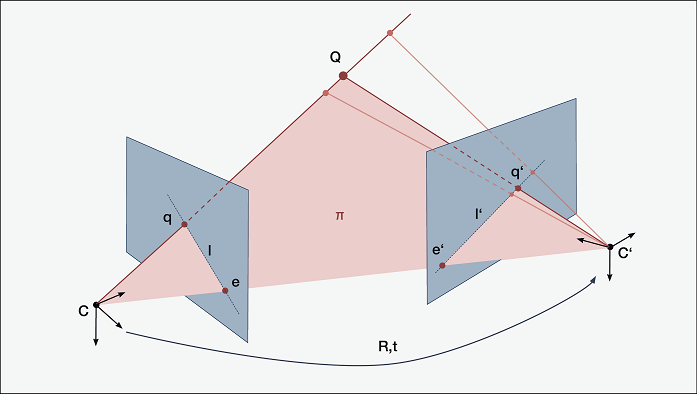
\includegraphics[height=5cm]{nc.png}\\[1cm]
\end{center}

According to the camera model, each of the landmarks $Q$ will be projected onto 2-D plane of pixels as $q, q^{\prime}$. Motion, described by the rotation matrix $R$ and transformation vector $t$ can be reproduced than via Epipolar constraint. 

Pixel points $q, q^{\prime}$ are described by the following equations:
\begin{equation}
    \begin{cases}
      s_{1} p_{1} = K P\\
      s_{2} p_{2} = K(RP + t)
    \end{cases}\,.
\end{equation}

As was discussed in the setting, due to the limitations of the approach, we can represent the points only to some constant factor. Moreover, it is worth mentioning that $p_{1}, p_{2}$ will be the points matched by the feature matcher.

To find the coordinates on the normalized plane of two pixels, we can simply take the inverse of the matrix representing a camera:
$x_{1, 2} = K^{-1}p_{1, 2}.$ Then the equation above can be rewritten as $x_{2} = Rx_{1} + t.$ This can be further transformed into $$p_{2}^{\italic{T}} K^{-T} t \times R K^{-1} p_{1} = 0.$$ This equation is referred to as epipolar constraint. For the sake of simplicity, the notions of Fundamental and Essential matrices are introduced:
\begin{equation}
    \begin{cases}
      E = t \times R\\
      F = K^{-T} t \times R K^{-1}\\
      x_{2}^{\italic{T}} E x_{1} = 0\\
      p_{2}^{\italic{T}} F p_{1} = 0
    \end{cases}\,.
\end{equation}

It is clear that usage of Essential matrix will make the calculations more accurate, as it uses precomputed calibration parameters for the camera. 
The process of camera pose estimation can then be summarized as:
\begin{enumerate}
    \item Find $E$ or $F$ from the known pixel positions.
    \item Find $R$, $t$ based on those matrices.
\end{enumerate}

In practice, the Essential matrix is found via Eight-Point algorithm and then $R, t$ are found via SVD and triangulation to get the result that would satisfy the constraints given by the known projections of landmarks.

\begin{equation}
    \begin{cases}
        R = U R_{Z(\pm pi/2)} V^{T}\\
        t = U R_{Z(\pm pi/2)} \Sigma U^{T}
    \end{cases}\,.
\end{equation}


\subsection{Triangulation}


\section{Overview of approaches}

\section{Implementation}

\begin{algorithm}[H]
	\KwData{stream of video frames}

	initialization\;
	calibrate camera\;
	\While{true}{
		get frame\;
		
		get the features\;
		match the features between current and previous frame\;
		
		find essential matrix\;
		
		find rotation matrix and transformation\;
		
		store the movement and point map\;
		
		update previous frame\;
	}
	\caption{General algorithm of SLAM}
\end{algorithm}

\vskip 1cm

The algorithm was implemented in Python via pyopencv. The visualizer of the SLAM was written via OpegGL. For the feature extraction the ORB was used due to its computational efficiency. Feature matching was done in brute-force manner because limitation on the number of features was only several hundreds. Fundamental matrix was then constructed as we lack the camera parameters for the test video. 

\begin{center}
    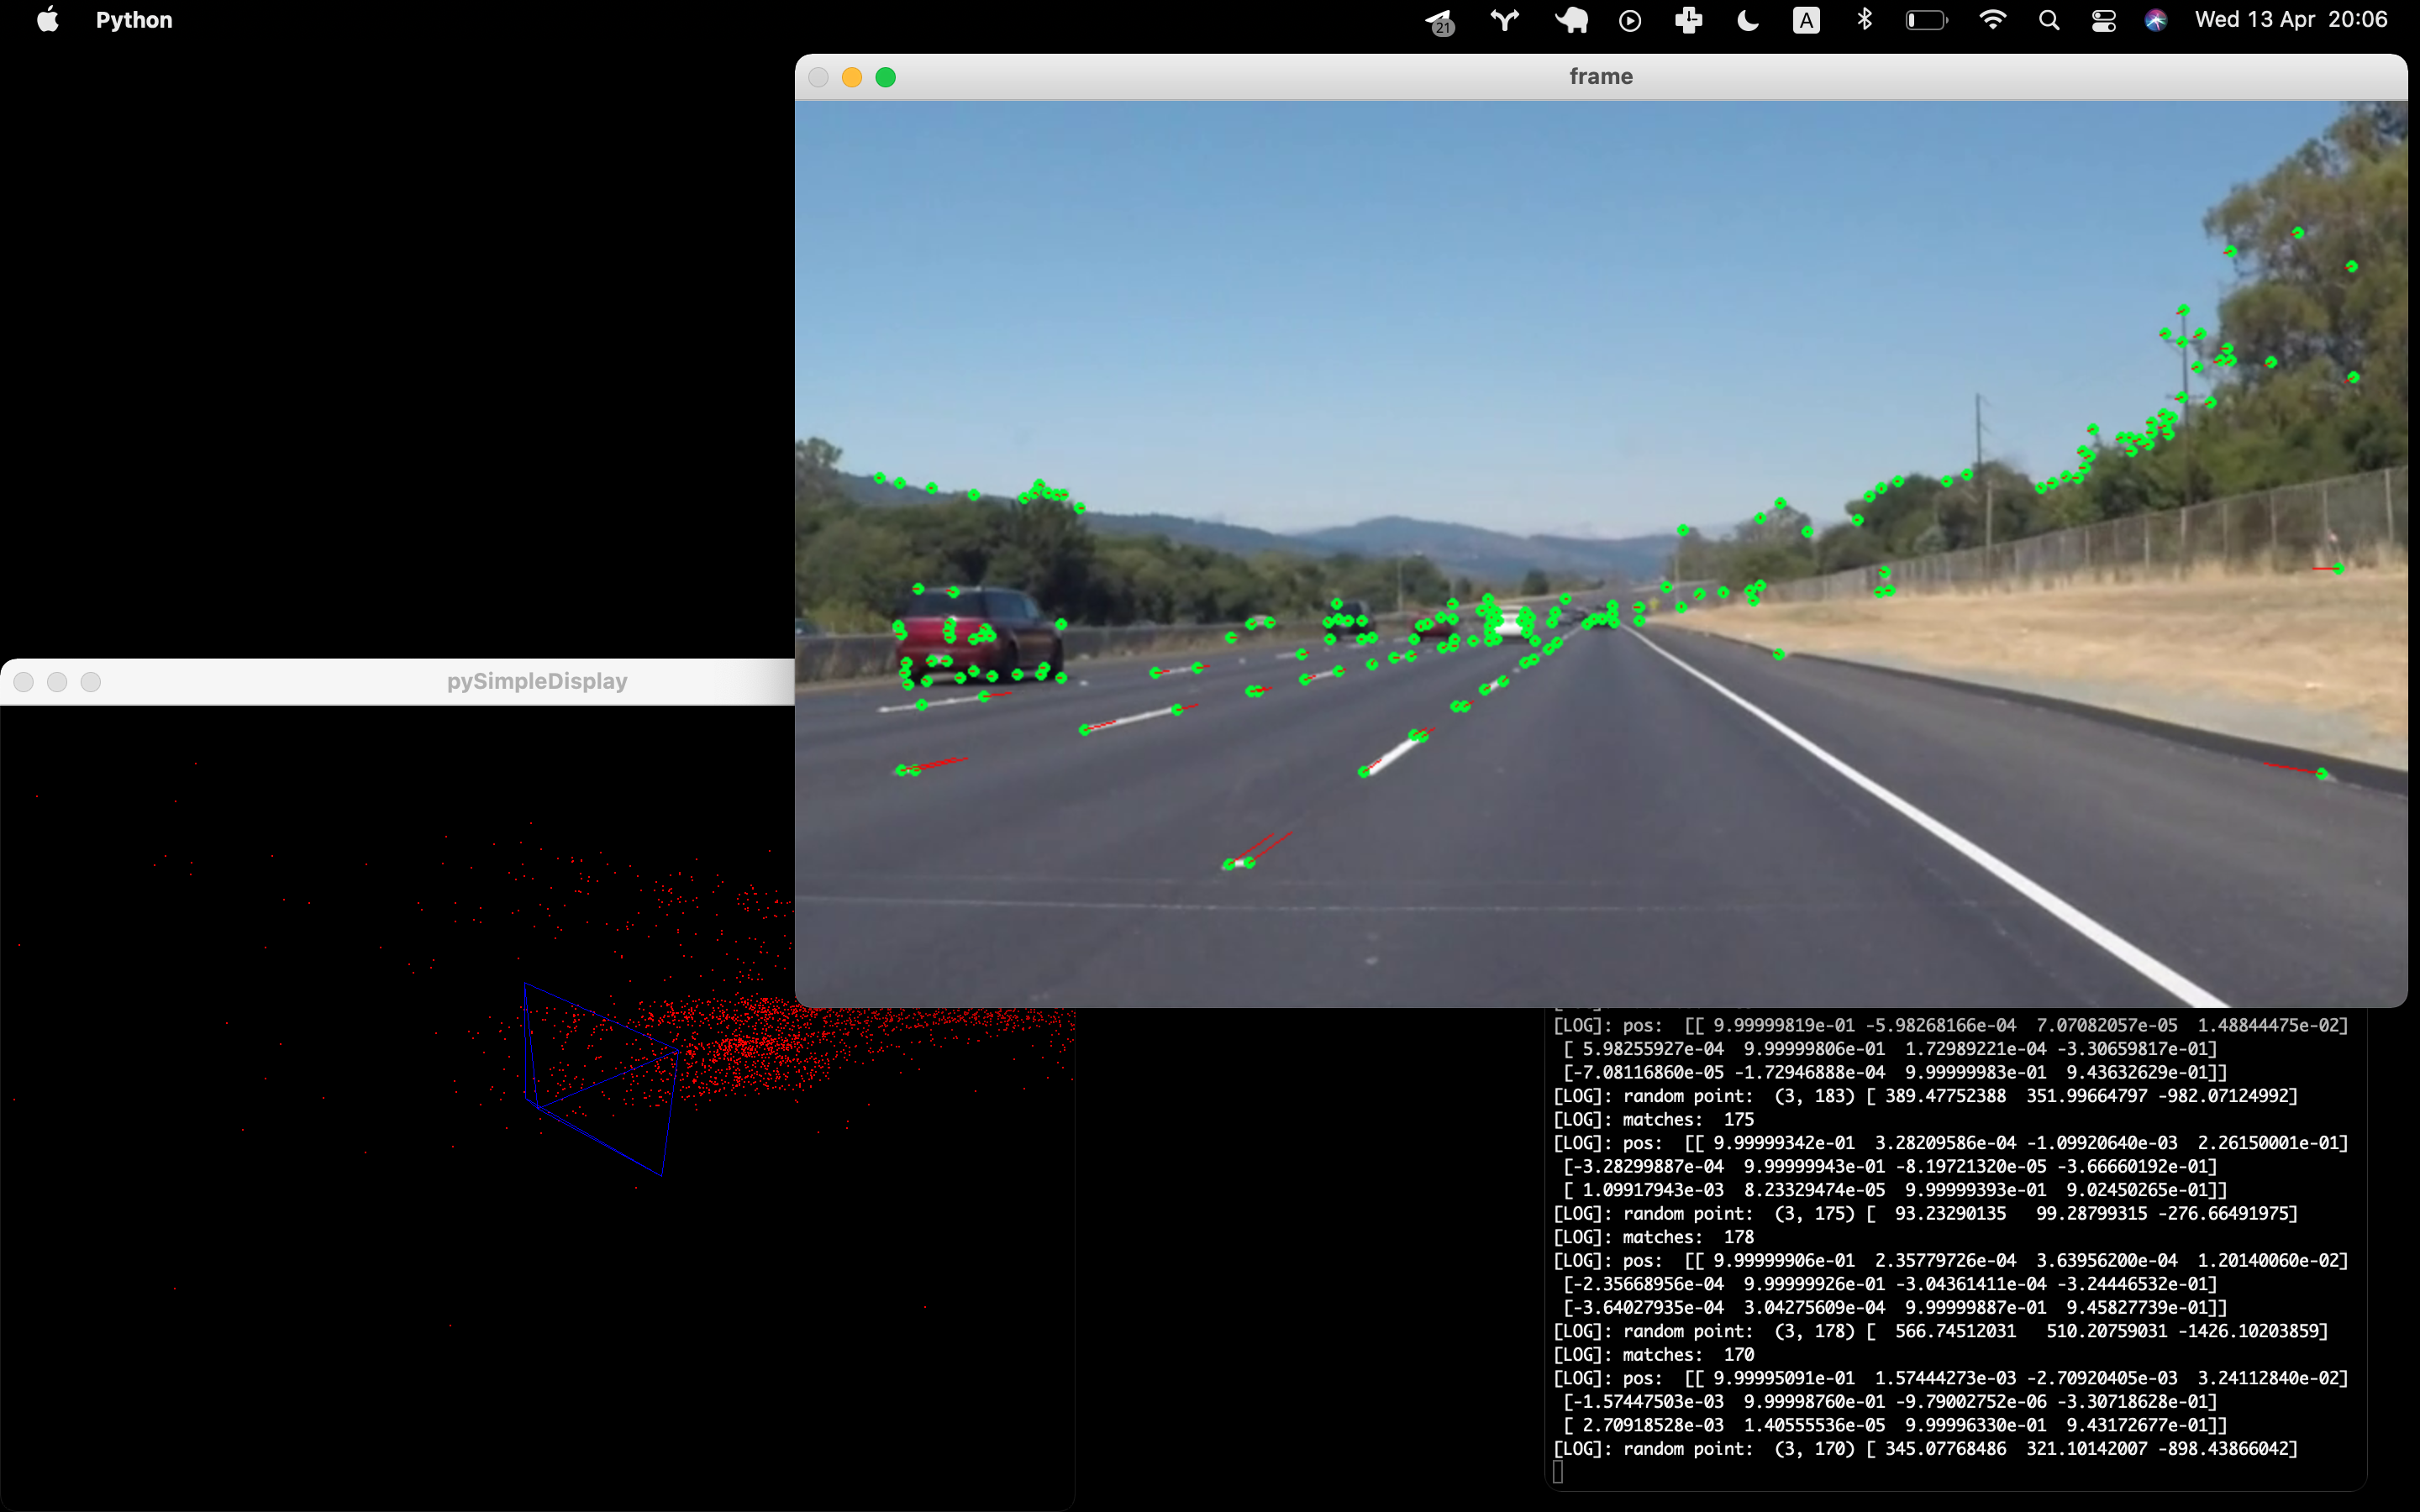
\includegraphics[height=10cm]{res.png}\\[1cm]
\end{center}

\section{Experiments}

\section{Limitations}

There are two main limitations of such approach:
\begin{enumerate}
    \item Triangulation is only possible if the enough amount of translation is present. If the amount of translation is small, pixel's change would result in big depth uncertainty. On the other hand, if translation is too big, the algorithm may fail to match the features. This problem will be especially seen in cases of so-called pure rotation, when there is no translation. Though in not so extreme cases, there are means to make this problem less visible - delayed triangulation etc.
    \item Assumption about static sight of view brings a lot of limitations as well.  For instance, the algorithm cannot be applied to autopilots as the moving object would make it think that the camera has moved. 
\end{enumerate}

\section{Conclusions}

\appendix

\begin{thebibliography}{9}

\bibitem{GitHub} \texttt{https://github.com/bohdanhlovatskyi/OhISee}

\end{thebibliography}

\end{document}